\begin{frame}
	\frametitle{Tandem Diels-Alder Cycloaddition}
	\begin{figure}
		\centering
		\includegraphics[width=1.0\linewidth]{fig/tand-diels-module}
		\caption{A Module Figure}
		\label{fig:tand-diels-module}
	\end{figure}
	
	
	The diastereoselectivity of this two-step process is
	very high, that is why this process is very important for generating
	multiple stereocentres from rather simple starting materials.\footfullcite{RN8}
	
\end{frame}

\begin{frame}
	\frametitle{A Synthetic Example\footfullcite{cannillo2013fast}}
	\begin{figure}
		\centering
		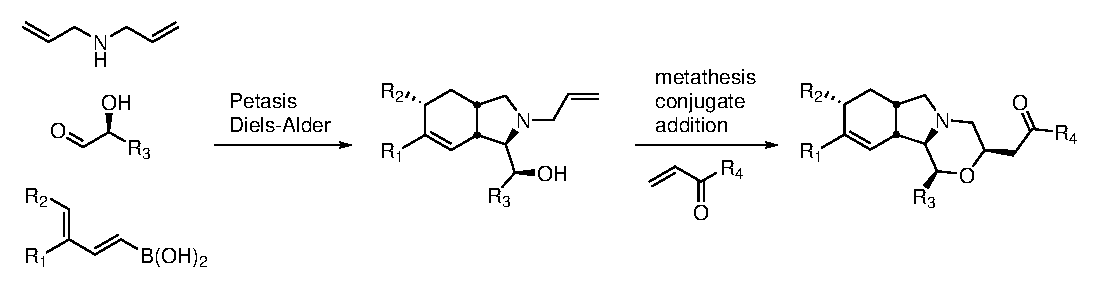
\includegraphics[width=1.0\linewidth]{fig/tand-diels-example}
		\caption{}
		\label{fig:tand-diels-example}
	\end{figure}
	
\end{frame}